
%(BEGIN_QUESTION)
% Copyright 2014, Tony R. Kuphaldt, released under the Creative Commons Attribution License (v 1.0)
% This means you may do almost anything with this work of mine, so long as you give me proper credit

One of the resistors in this voltage divider circuit is failed (either open or shorted).  Based on the voltage readings shown at each load, determine which one and what type of failure it is:

$$\includegraphics[width=15.5cm]{i01136x01.eps}$$

\underbar{file i01136}
%(END_QUESTION)





%(BEGIN_ANSWER)

Resistor R1 has failed (partially) shorted.  We can tell this because both loads \#2 and \#3 are being over-powered.

%(END_ANSWER)





%(BEGIN_NOTES)

Discuss with your students how they were able to predict R1 was the faulty resistor.  Is there any particular clue in the diagram indicating R1 as the obvious problem?  Some students may suspect an open failure in resistor R3 could cause the same effects, but there is a definite way to tell that the problem can {\it only} come from a short in R1 (hint: analyze resistor R2). 

Explain that not all ``shorted'' failures are ``hard'' in the sense of being direct metal-to-metal wire connections.  Quite often, components will fail shorted in a ``softer'' sense, meaning they still have some non-trivial amount of electrical resistance.

%INDEX% Electronics review: series-parallel circuits

%(END_NOTES)


